\setcounter{figure}{2}

\begin{frame}
    \begin{figure}
        \centering
        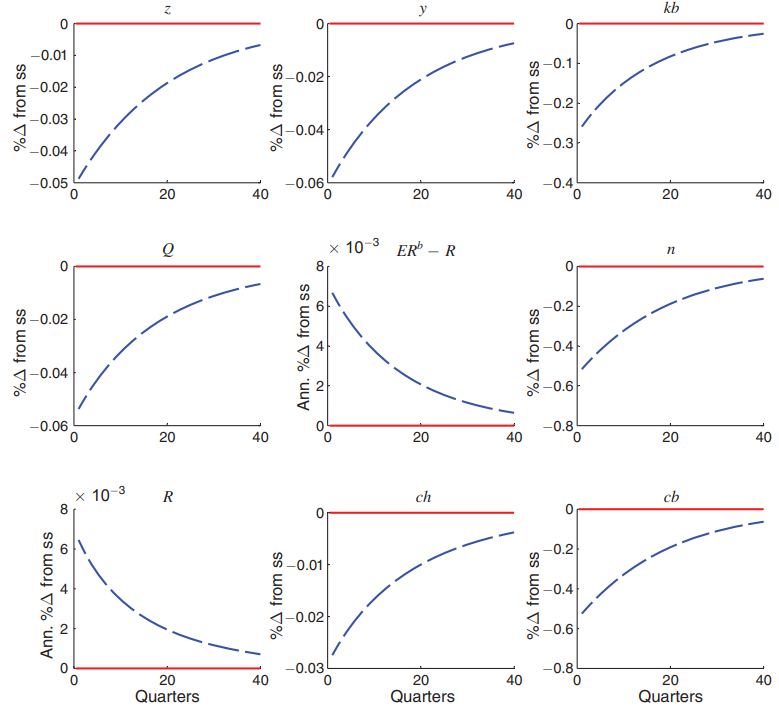
\includegraphics[height = 0.9\textheight]{fig/fig3.png}
        \caption{A Recession in the Baseline Model: No Bank Run Case}
    \end{figure}
\end{frame}

\begin{frame}
    \begin{figure}
        \centering
        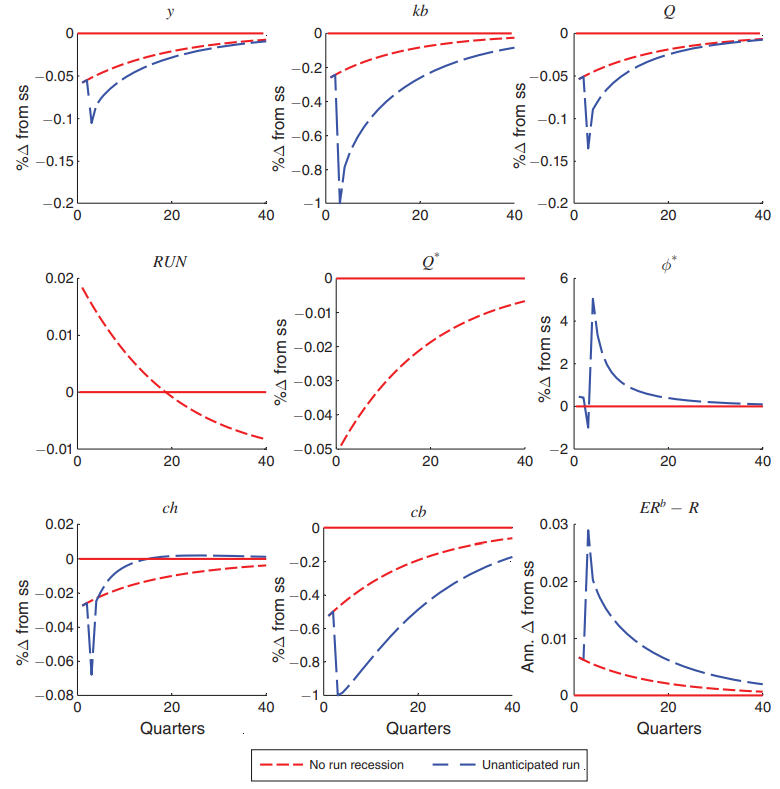
\includegraphics[height = 0.9\textheight]{fig/fig4.png}
        \caption{Ex Post Bank Run in the Baseline Model}
    \end{figure}
\end{frame}

\begin{frame}
    \begin{figure}
        \centering
        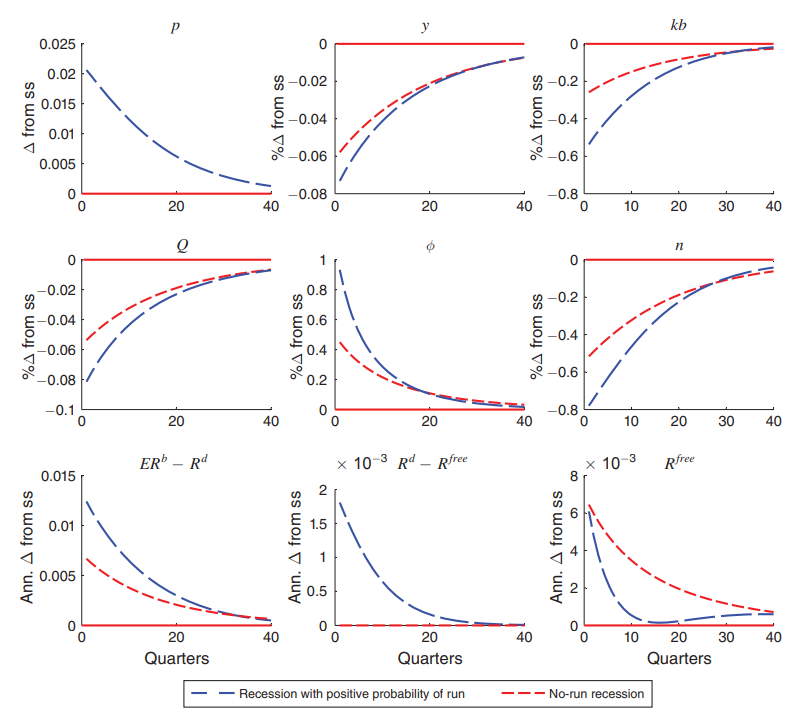
\includegraphics[height = 0.9\textheight]{fig/fig5.png}
        \caption{Recession with Positive Probability of a Run}
    \end{figure}
\end{frame}

\begin{frame}
    \begin{figure}
        \centering
        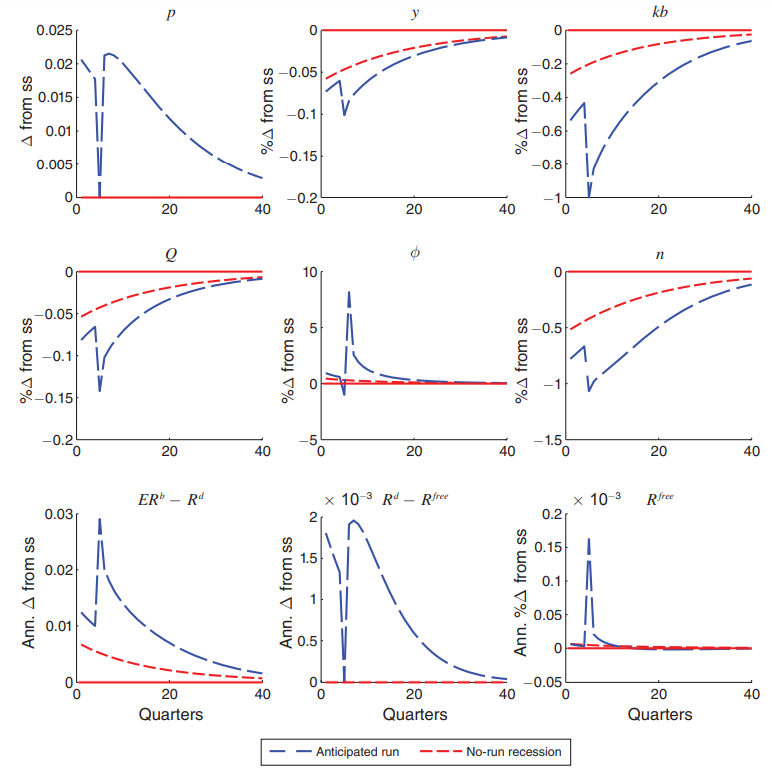
\includegraphics[height = 0.9\textheight]{fig/fig6.png}
        \caption{Recession with Positive Probability of a Run}
    \end{figure}
\end{frame}

\begin{frame}
    \begin{figure}
        \centering
        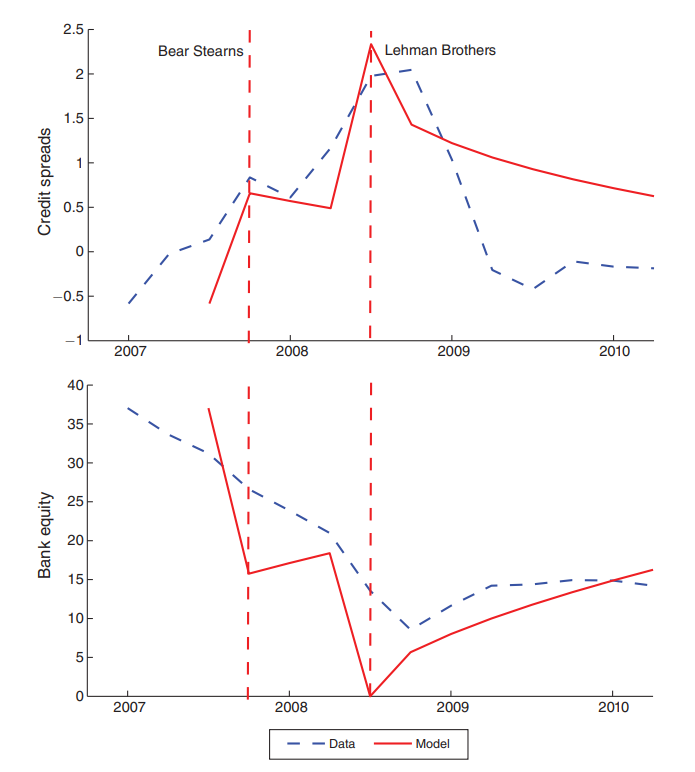
\includegraphics[height = 0.9\textheight]{fig/fig7.png}
        \caption{Recession with Positive Probability of a Run}
    \end{figure}
\end{frame}